\section{definition12(for the main theorem)}
\begin{definition}
\end{definition}

Suppose we have a braid diagram as follows :

\begin{figure}[H] % Optional: [h] means here, [t] for top, [b] for bottom, [p] for page of floats
    \centering
    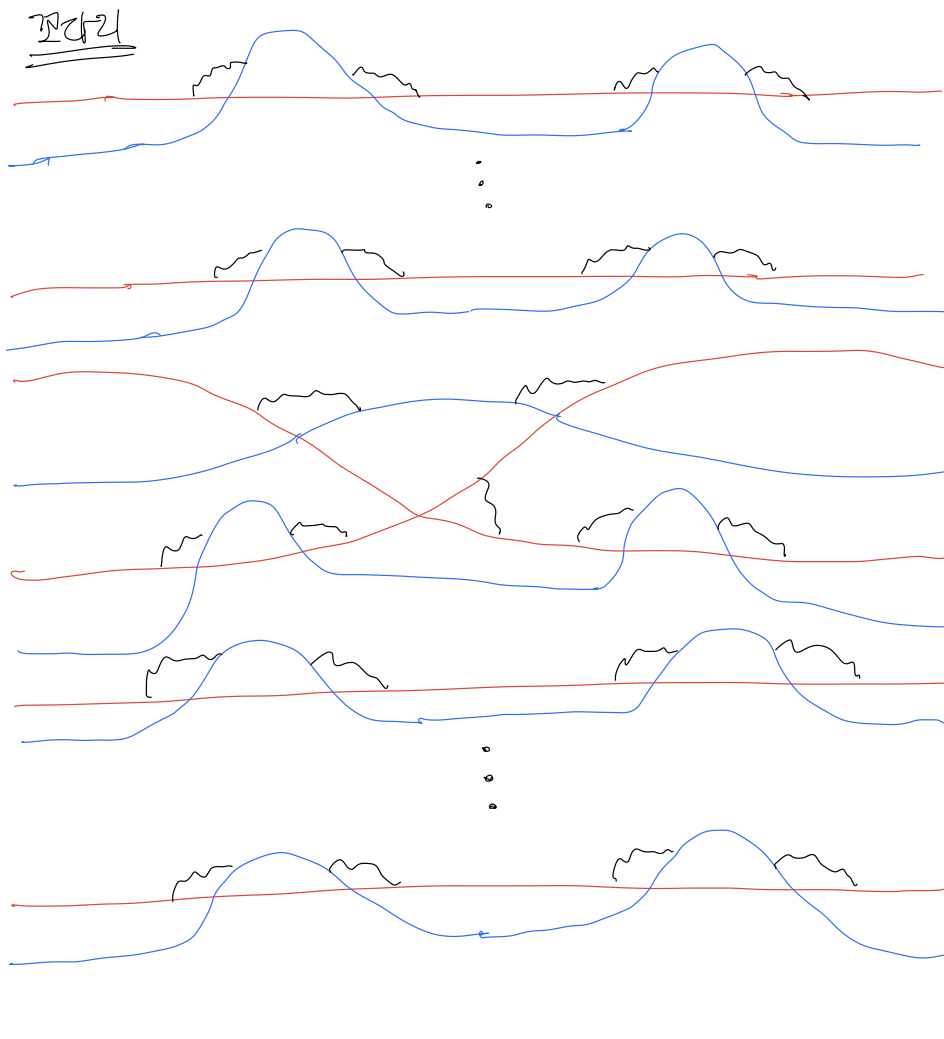
\includegraphics[width=\linewidth]{diagrams/definition12/1.png} % Adjust the width as needed
    \caption{Your caption here}
    \label{fig:your-label}
\end{figure}

We define MOVE \RN{12} so that the final diagram looks as follows :

\begin{figure}[H] % Optional: [h] means here, [t] for top, [b] for bottom, [p] for page of floats
    \centering
    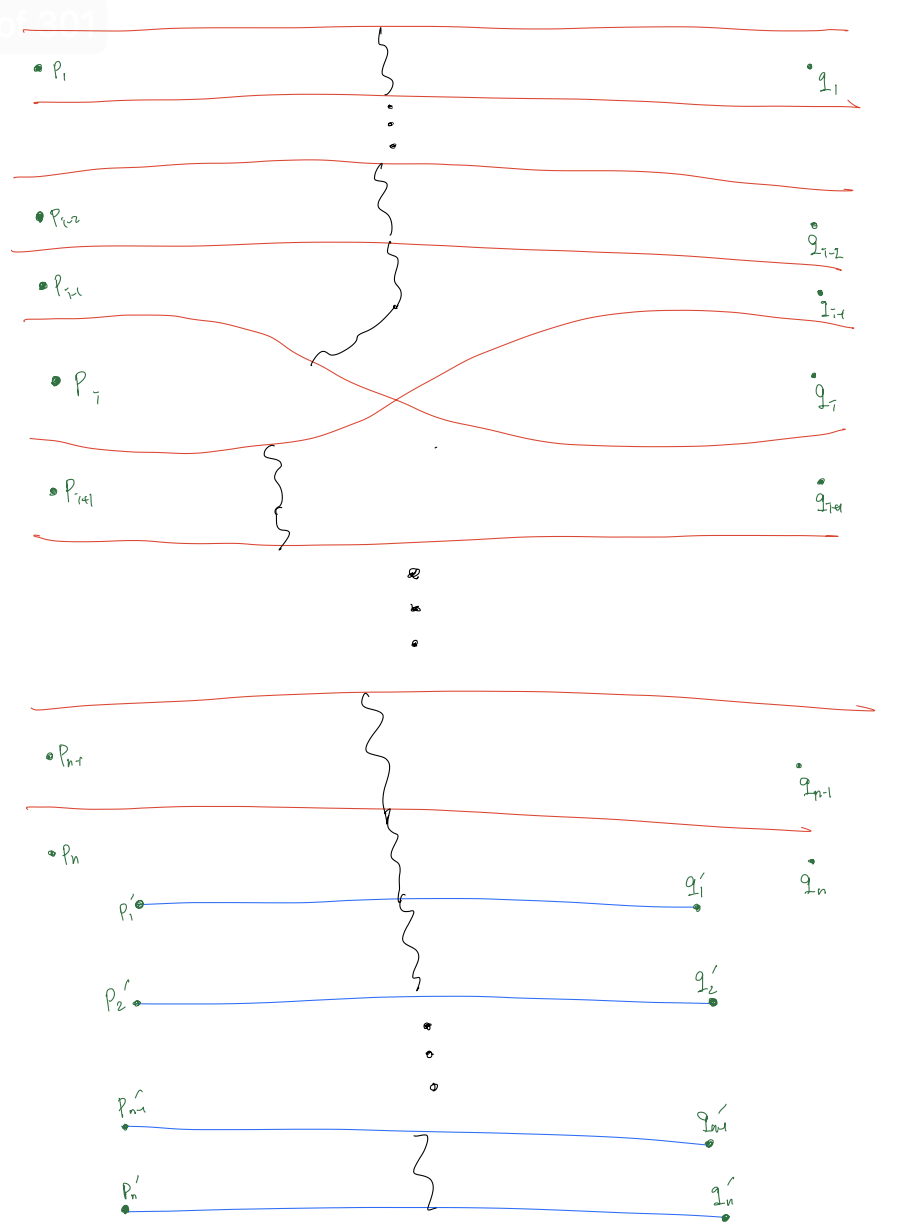
\includegraphics[width=\linewidth]{diagrams/definition12/2.png} % Adjust the width as needed
    \caption{Your caption here}
    \label{fig:your-label}
\end{figure}

We define MOVE \RN{12} as follows :

(Step1) Apply MOVE \RN{2} to the region inside the purple circle :

\begin{figure}[H] % Optional: [h] means here, [t] for top, [b] for bottom, [p] for page of floats
    \centering
    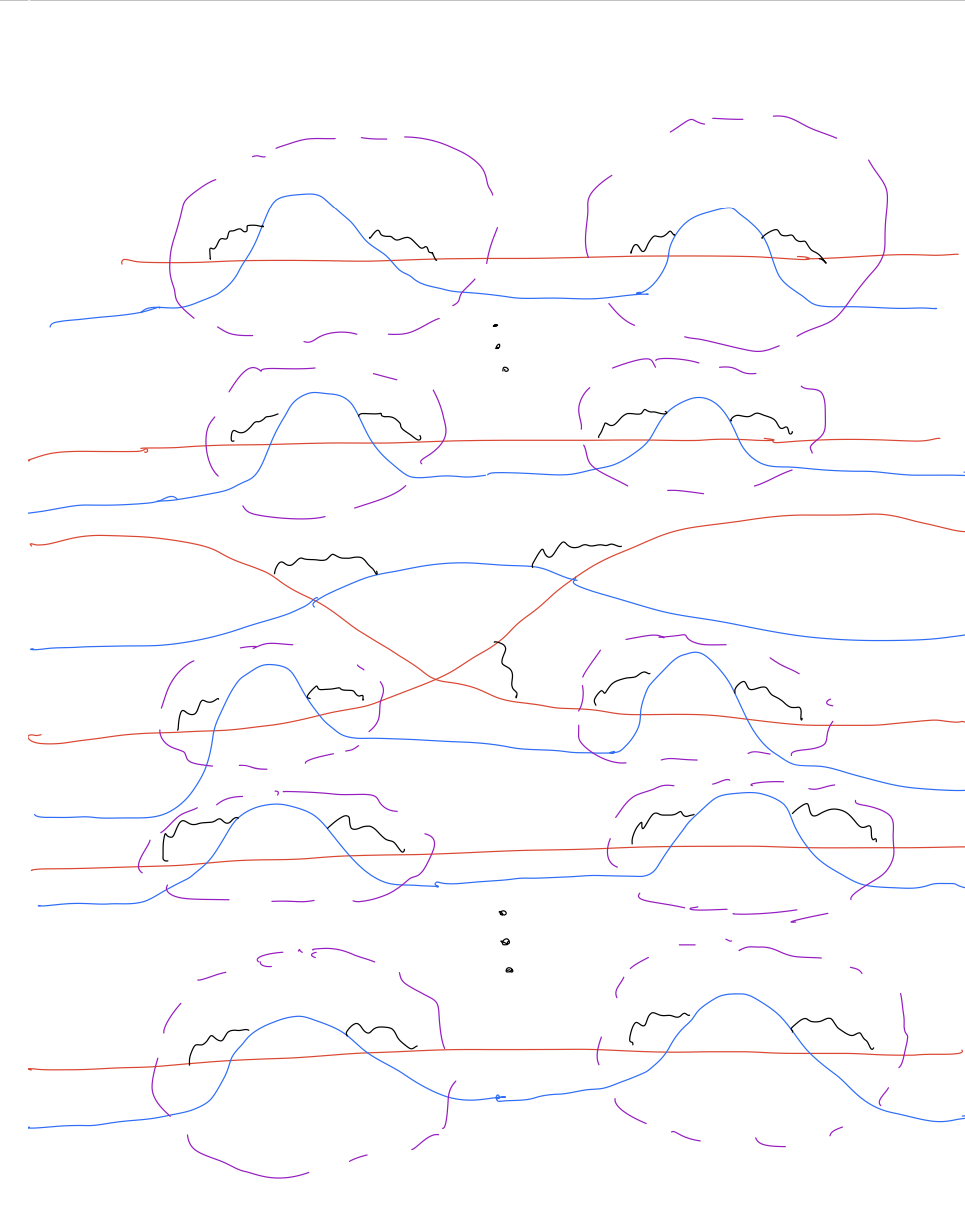
\includegraphics[width=\linewidth]{diagrams/definition12/3.png} % Adjust the width as needed
    \caption{Your caption here}
    \label{fig:your-label}
\end{figure}

we get :

\begin{figure}[H] % Optional: [h] means here, [t] for top, [b] for bottom, [p] for page of floats
    \centering
    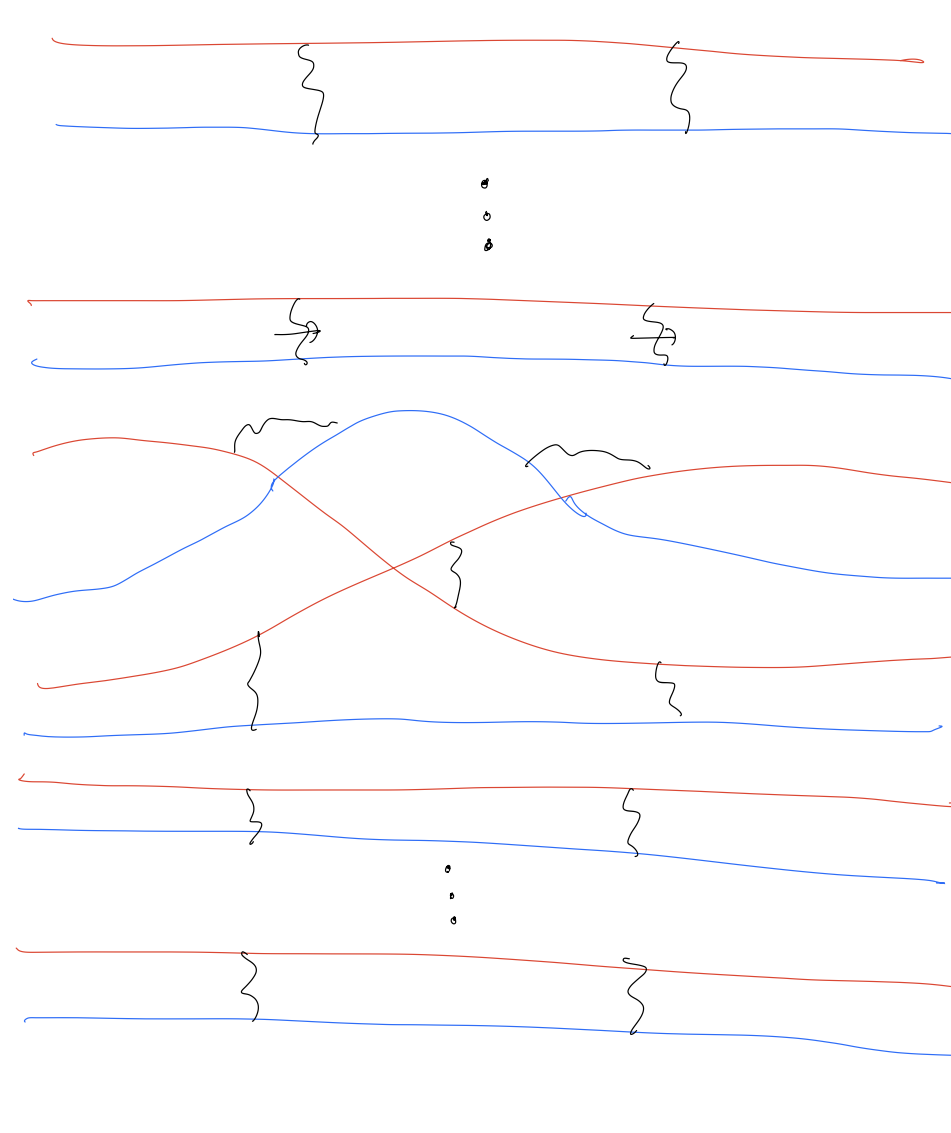
\includegraphics[width=\linewidth]{diagrams/definition12/4.png} % Adjust the width as needed
    \caption{Your caption here}
    \label{fig:your-label}
\end{figure}

(Step2)get rid of the squiggly lines in the region inside the purple circles:

\begin{figure}[H] % Optional: [h] means here, [t] for top, [b] for bottom, [p] for page of floats
    \centering
    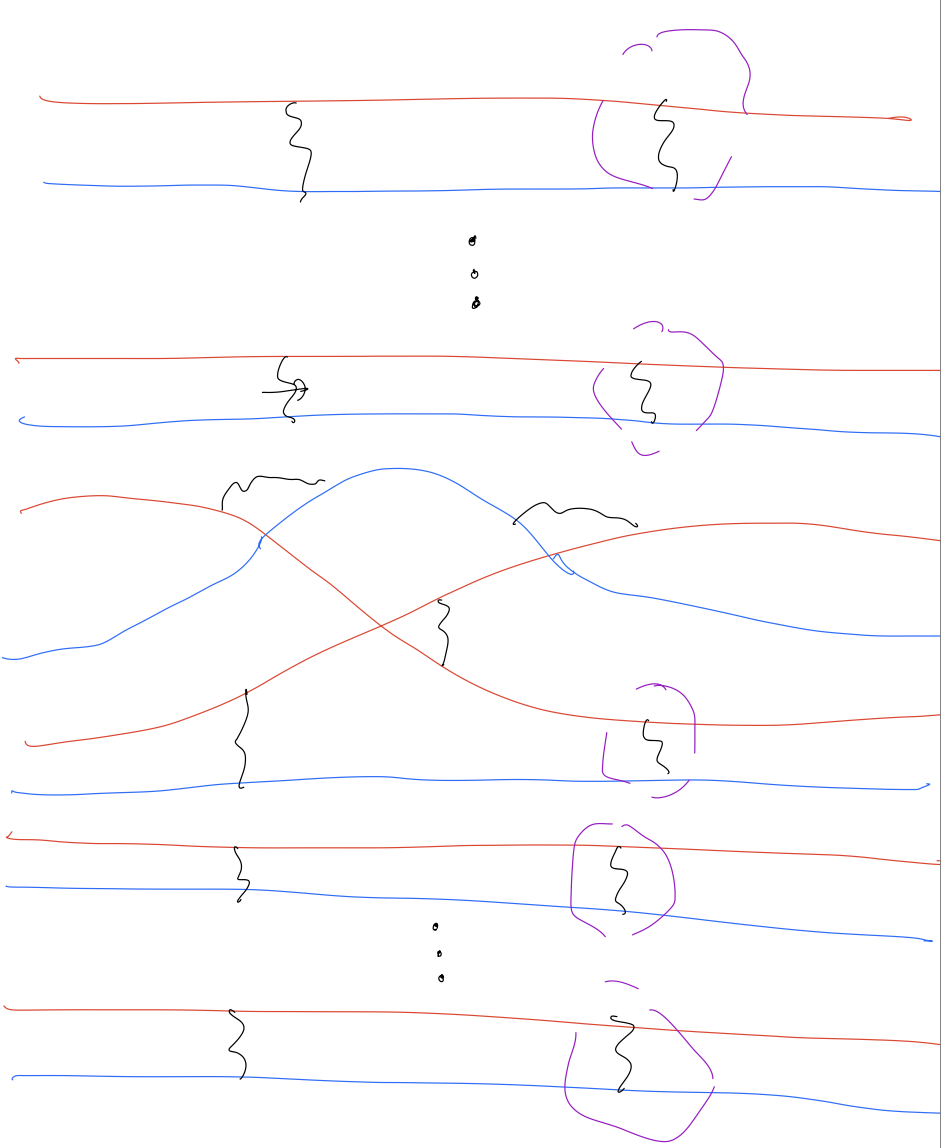
\includegraphics[width=\linewidth]{diagrams/definition12/5.png} % Adjust the width as needed
    \caption{Your caption here}
    \label{fig:your-label}
\end{figure}

we get :

\begin{figure}[H] % Optional: [h] means here, [t] for top, [b] for bottom, [p] for page of floats
    \centering
    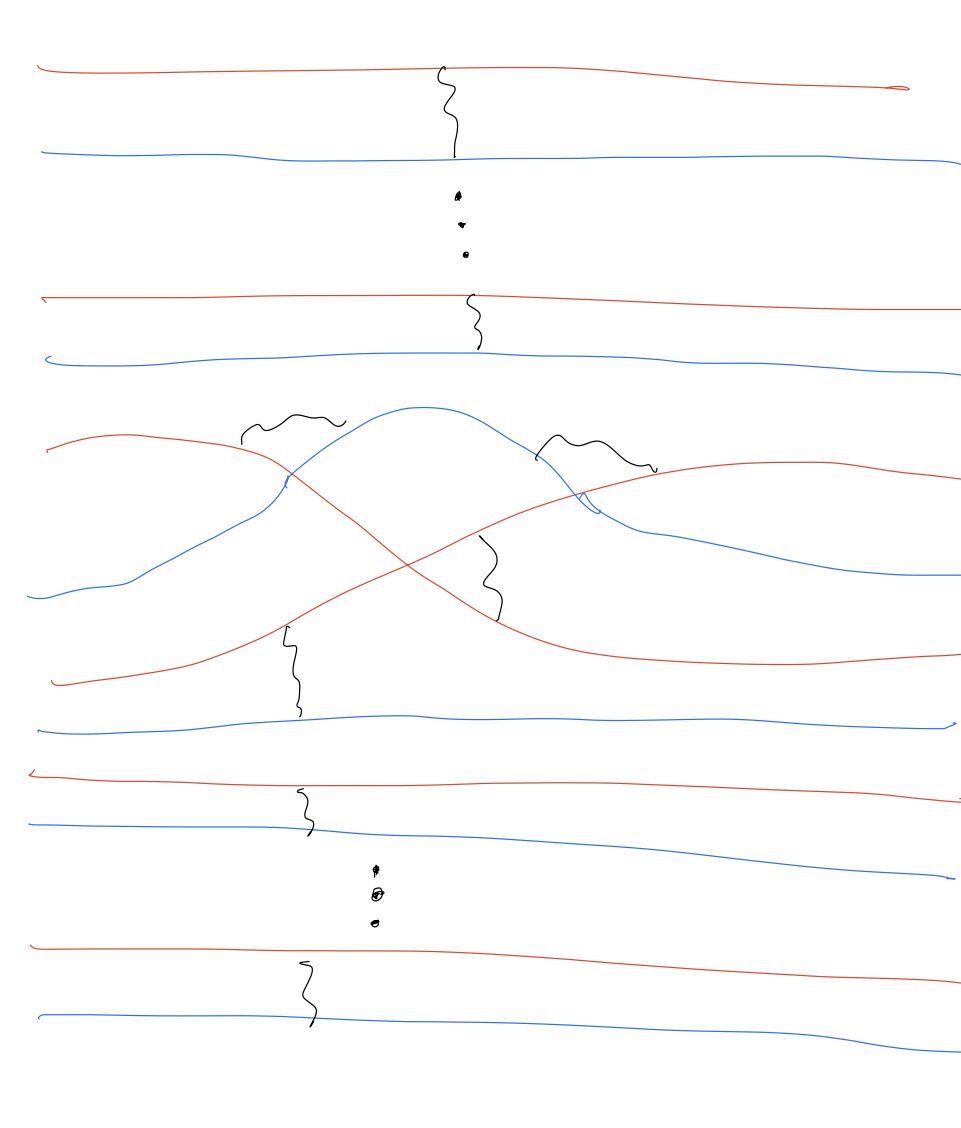
\includegraphics[width=\linewidth]{diagrams/definition12/6.png} % Adjust the width as needed
    \caption{Your caption here}
    \label{fig:your-label}
\end{figure}
(Step3) Apply MOVE \RN{7}-(a) to the region inside the purple circles

\begin{figure}[H] % Optional: [h] means here, [t] for top, [b] for bottom, [p] for page of floats
    \centering
    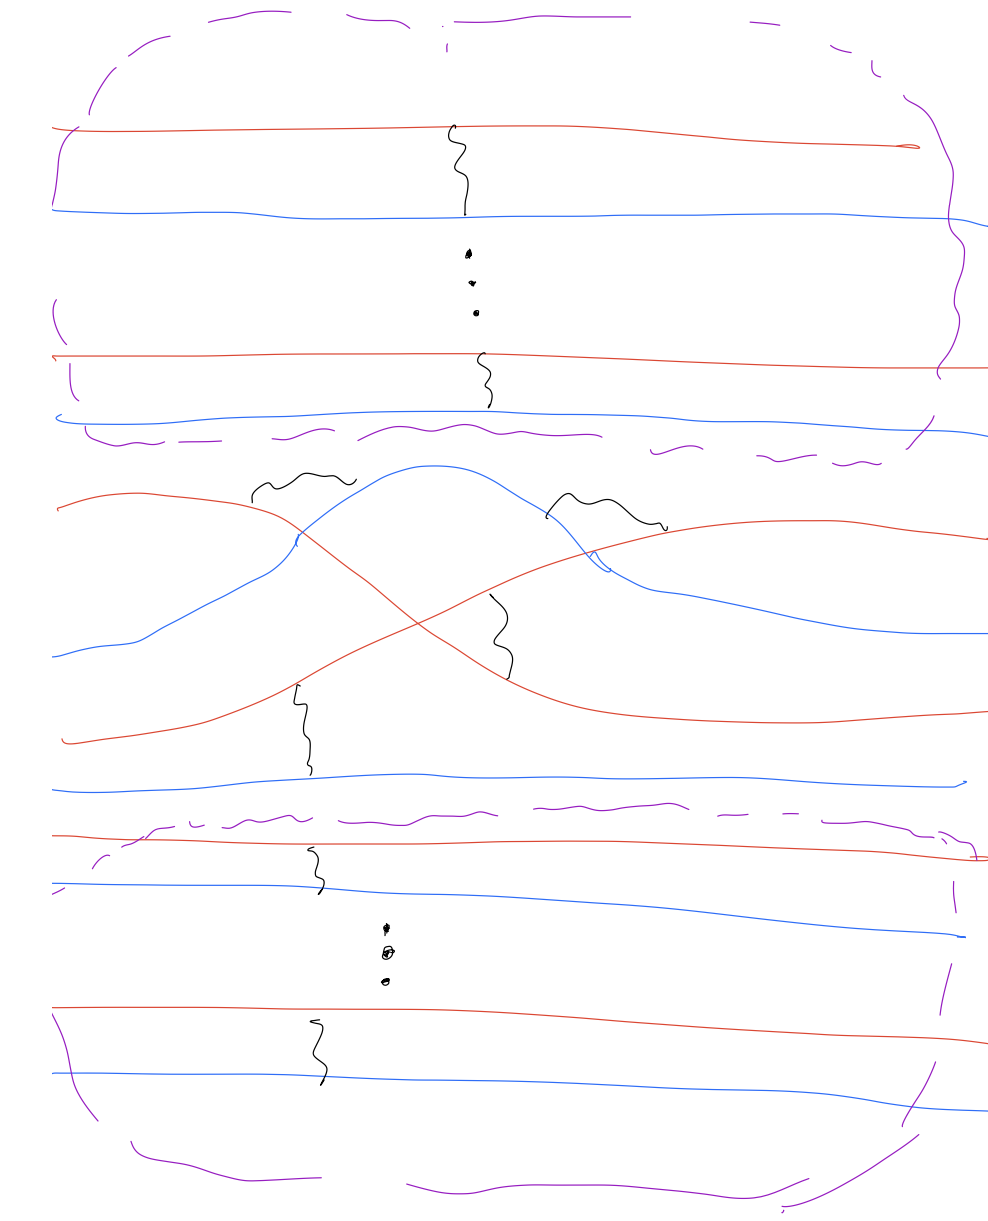
\includegraphics[width=\linewidth]{diagrams/definition12/7.png} % Adjust the width as needed
    \caption{Your caption here}
    \label{fig:your-label}
\end{figure}

we get :

\begin{figure}[H] % Optional: [h] means here, [t] for top, [b] for bottom, [p] for page of floats
    \centering
    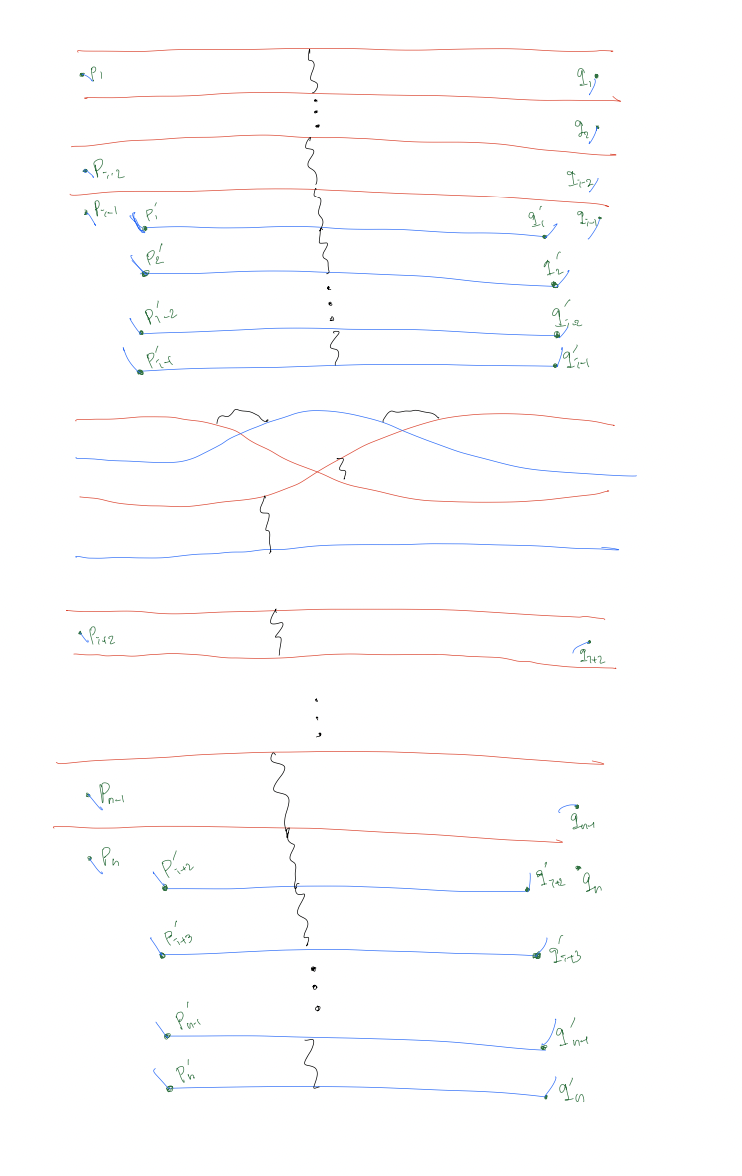
\includegraphics[width=\linewidth]{diagrams/definition12/8.png} % Adjust the width as needed
    \caption{Your caption here}
    \label{fig:your-label}
\end{figure}

(Step3') Apply MOVE \RN{7}-(b) to the region inside the purple circle

\begin{figure}[H] % Optional: [h] means here, [t] for top, [b] for bottom, [p] for page of floats
    \centering
    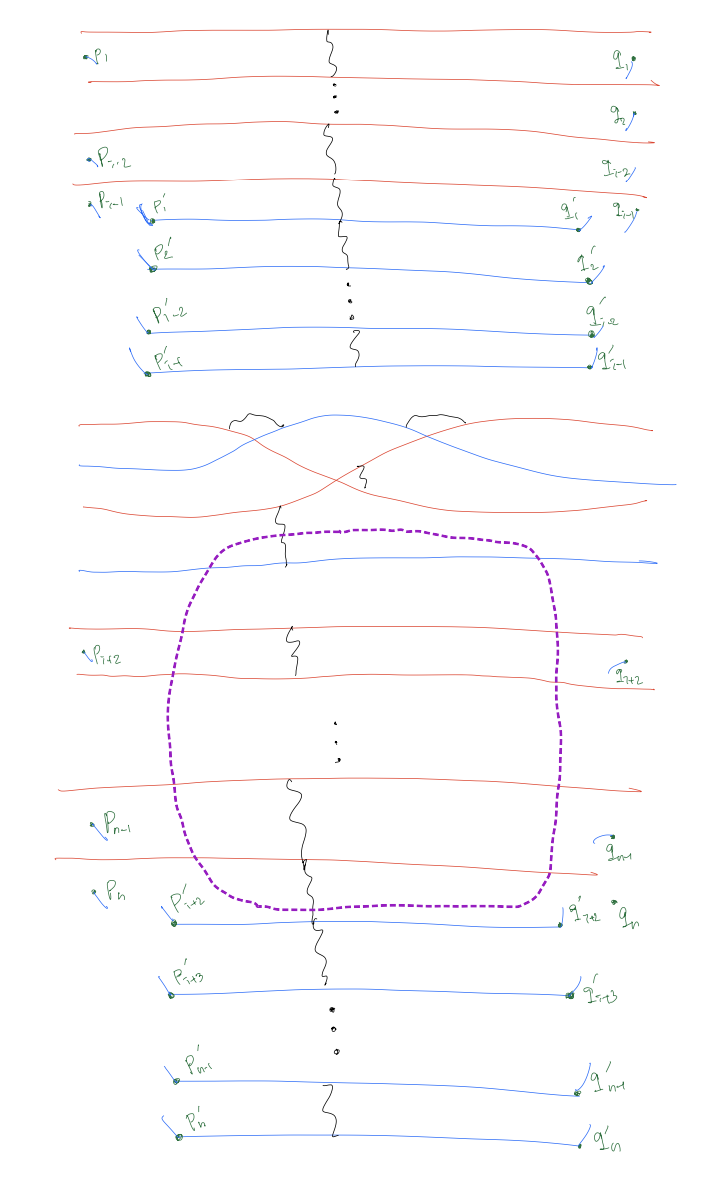
\includegraphics[width=\linewidth]{diagrams/definition12/9.png} % Adjust the width as needed
    \caption{Your caption here}
    \label{fig:your-label}
\end{figure}

we get:

\begin{figure}[H] % Optional: [h] means here, [t] for top, [b] for bottom, [p] for page of floats
    \centering
    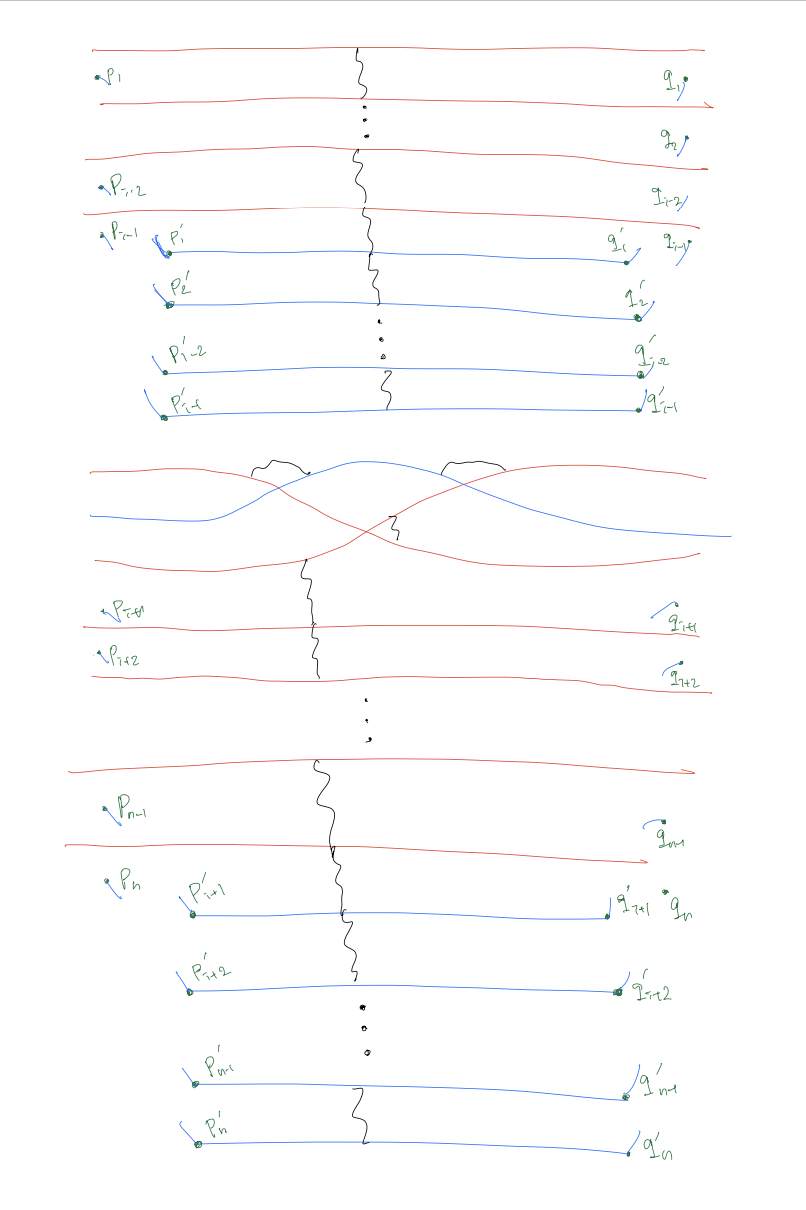
\includegraphics[width=\linewidth]{diagrams/definition12/10.png} % Adjust the width as needed
    \caption{Your caption here}
    \label{fig:your-label}
\end{figure}

(Step4) Appy MOVE \RN{9} to the region inside the purple circle

\begin{figure}[H] % Optional: [h] means here, [t] for top, [b] for bottom, [p] for page of floats
    \centering
    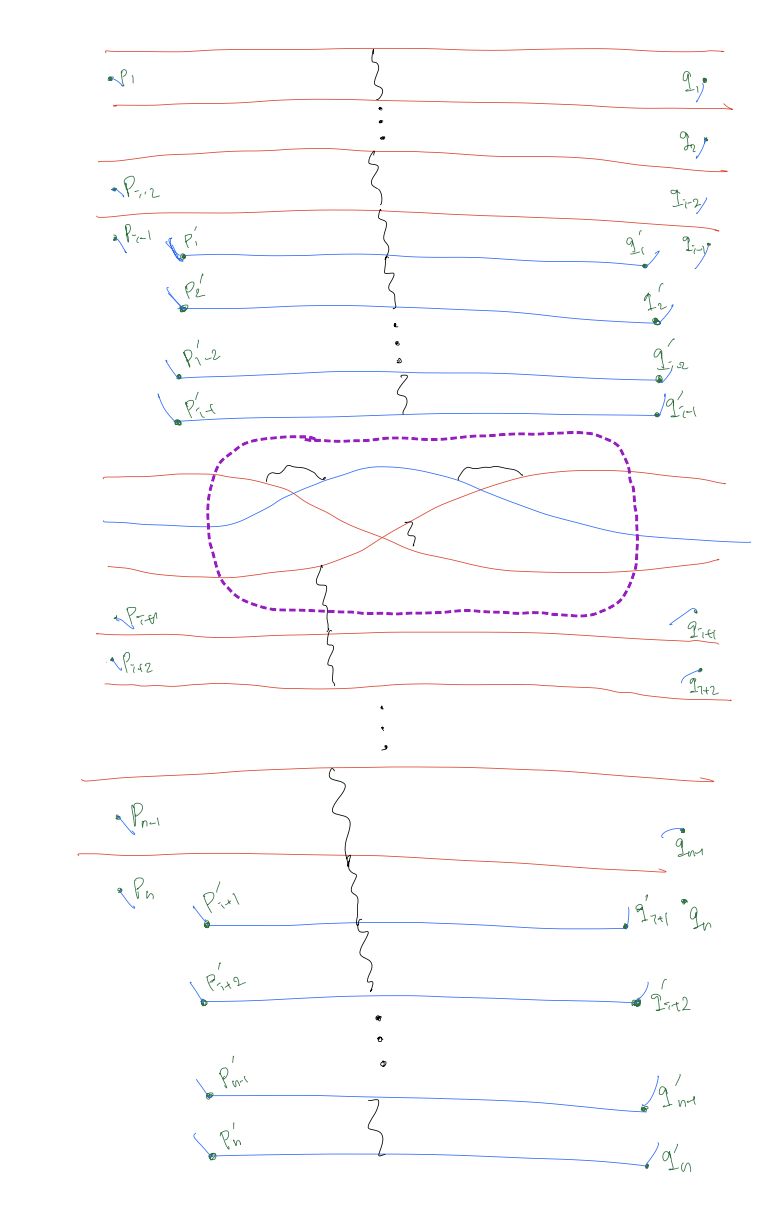
\includegraphics[width=\linewidth]{diagrams/definition12/11.png} % Adjust the width as needed
    \caption{Your caption here}
    \label{fig:your-label}
\end{figure}

we get :

\begin{figure}[H] % Optional: [h] means here, [t] for top, [b] for bottom, [p] for page of floats
    \centering
    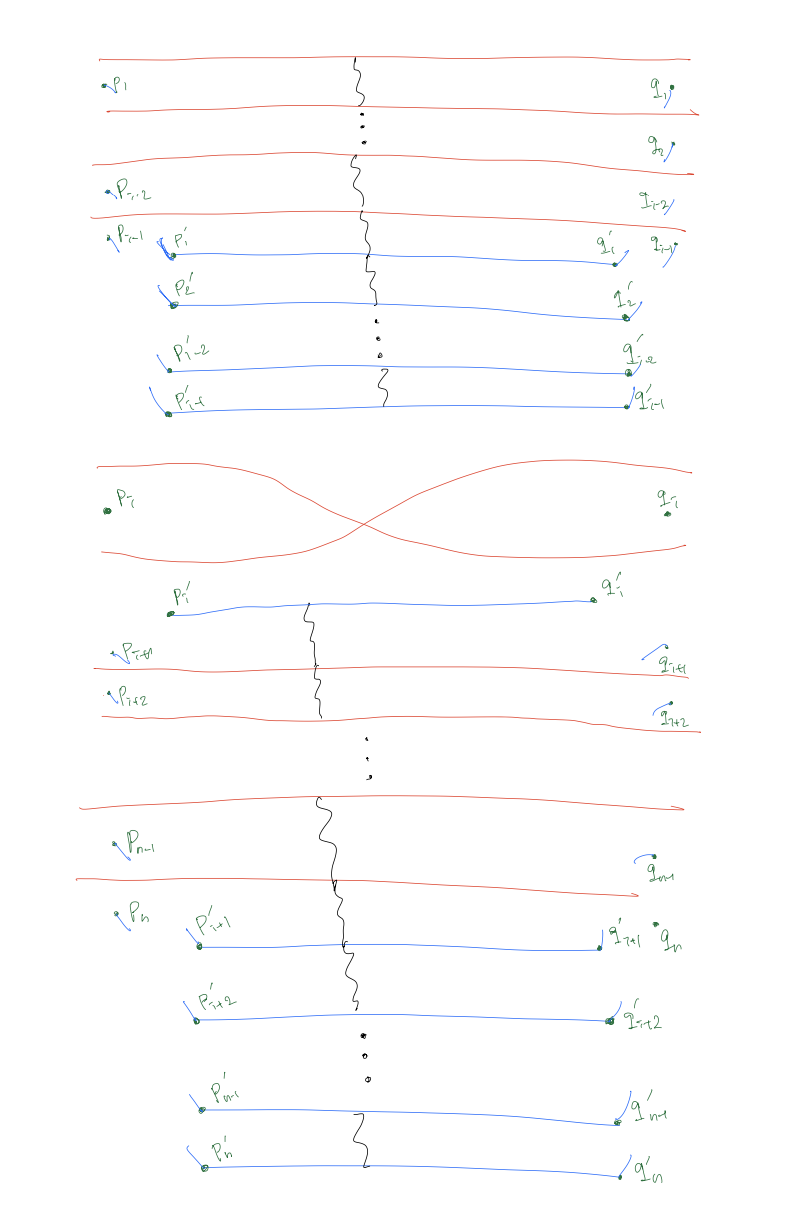
\includegraphics[width=\linewidth]{diagrams/definition12/12.png} % Adjust the width as needed
    \caption{Your caption here}
    \label{fig:your-label}
\end{figure}

(Step5) Apply MOVE \RN{11} to the region inside the purple circle

\begin{figure}[H] % Optional: [h] means here, [t] for top, [b] for bottom, [p] for page of floats
    \centering
    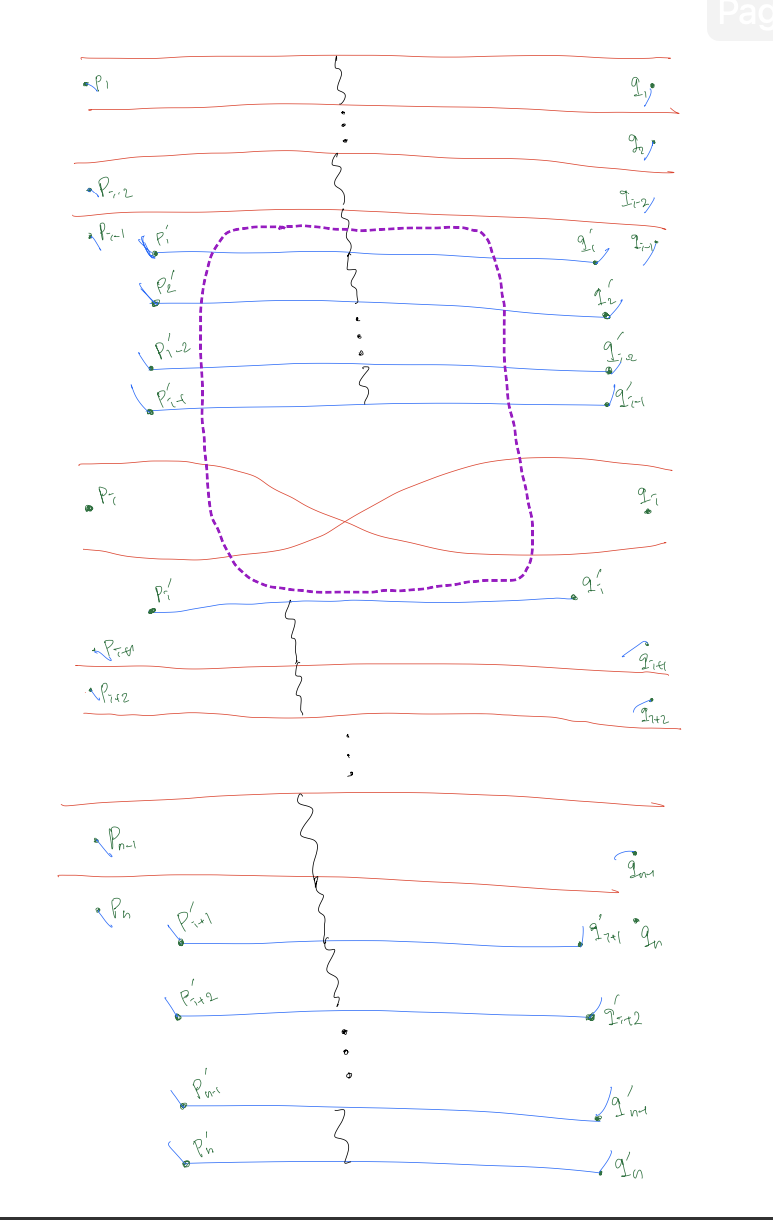
\includegraphics[width=\linewidth]{diagrams/definition12/13.png} % Adjust the width as needed
    \caption{Your caption here}
    \label{fig:your-label}
\end{figure}

we get :

\begin{figure}[H] % Optional: [h] means here, [t] for top, [b] for bottom, [p] for page of floats
    \centering
    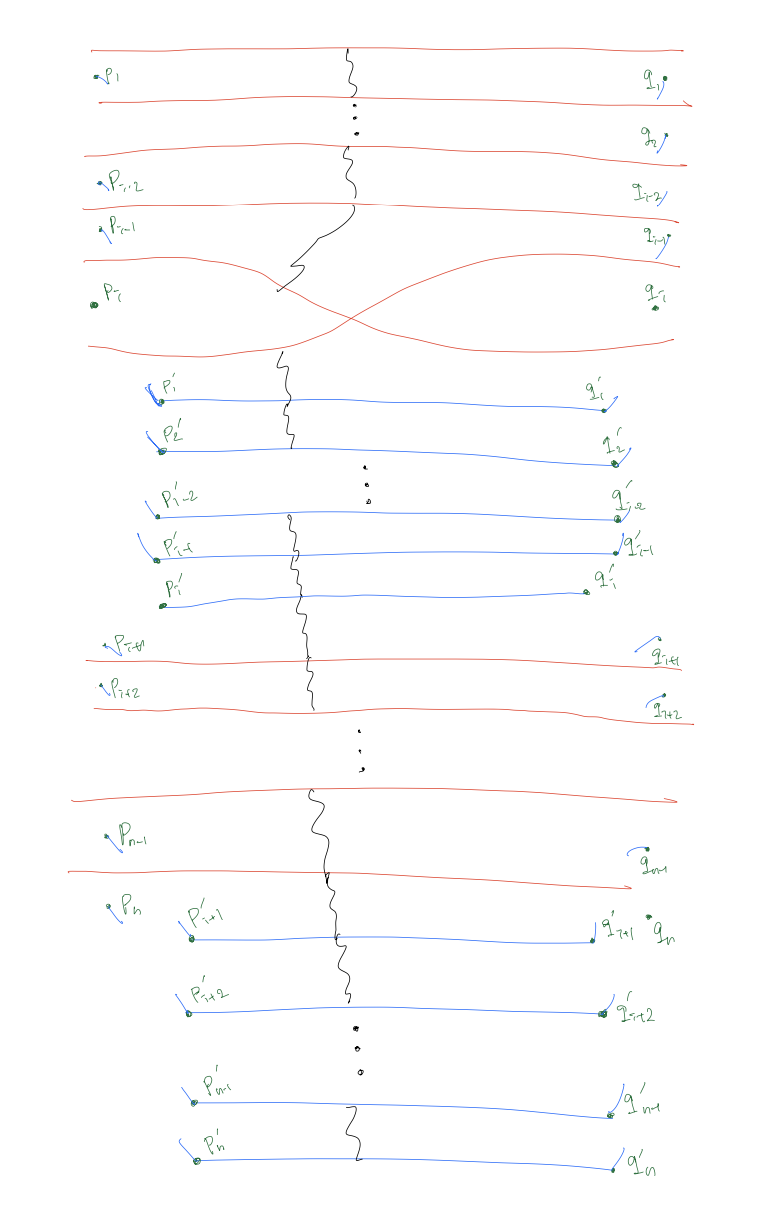
\includegraphics[width=\linewidth]{diagrams/definition12/14.png} % Adjust the width as needed
    \caption{Your caption here}
    \label{fig:your-label}
\end{figure}

(Step6) Apply MOVE \RN{7}-(b) to the region inside the purple circle

\begin{figure}[H] % Optional: [h] means here, [t] for top, [b] for bottom, [p] for page of floats
    \centering
    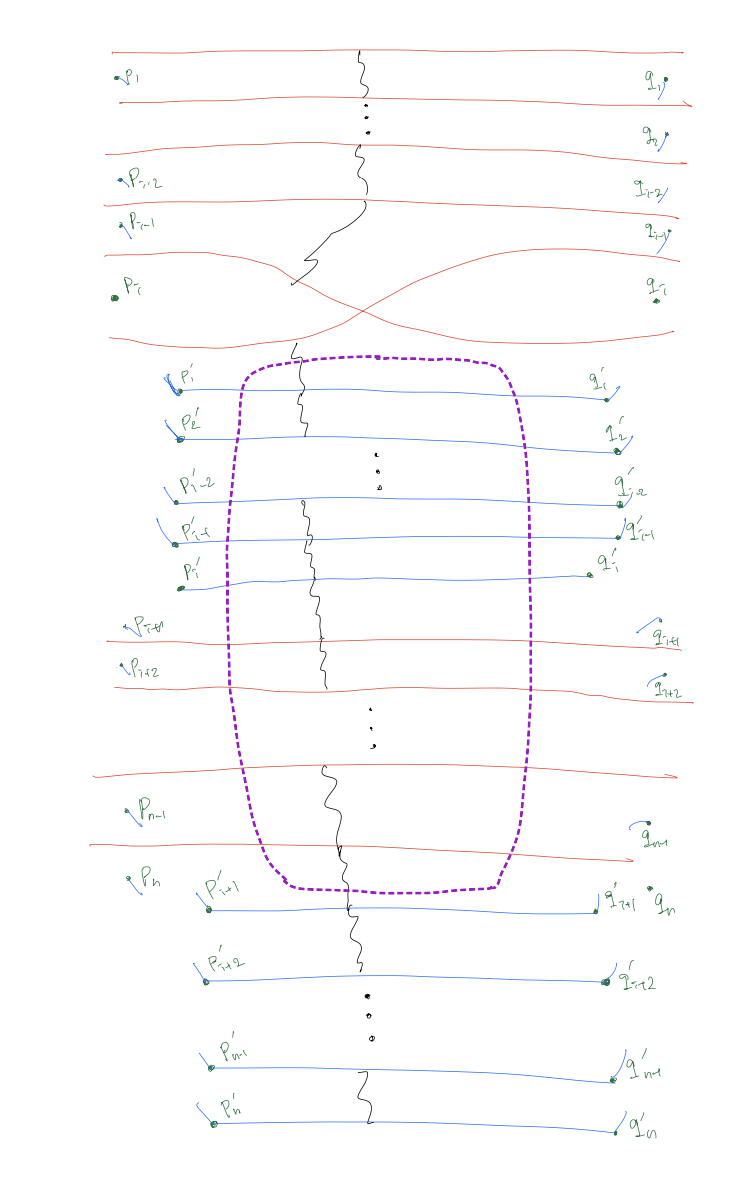
\includegraphics[width=\linewidth]{diagrams/definition12/15.png} % Adjust the width as needed
    \caption{Your caption here}
    \label{fig:your-label}
\end{figure}

we get :

\begin{figure}[H] % Optional: [h] means here, [t] for top, [b] for bottom, [p] for page of floats
    \centering
    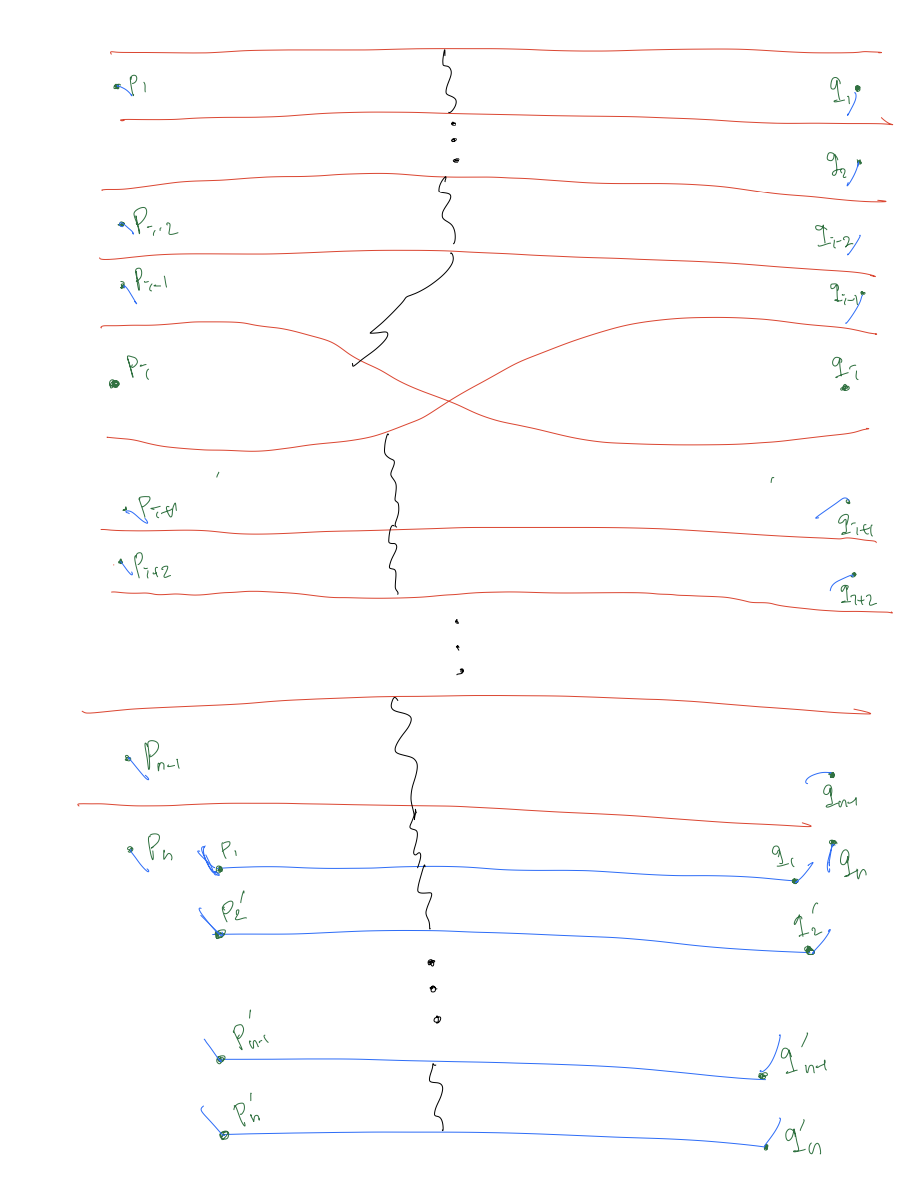
\includegraphics[width=\linewidth]{diagrams/definition12/16.png} % Adjust the width as needed
    \caption{Your caption here}
    \label{fig:your-label}
\end{figure}